\documentclass[a4paper,UTF8]{ctexart}

\usepackage{amsmath, amsthm, amssymb, amsfonts, hyperref, mathrsfs}%美国数学学会的包+?
\usepackage{geometry} %控制界面
\usepackage{bookmark}
\usepackage{fancyhdr} % header & footer
\usepackage{appendix} % 附录
\usepackage{tikz} %作图
\usepackage{graphicx} %插入图片的宏包
\usepackage{float} %设置图片浮动位置的宏包
\usepackage{subfigure} %插入多图时用子图显示的宏包
\usepackage{listings} %引用代码
\usepackage{physics,mathtools} %物理数学工具
\usepackage{comment}
\usepackage{framed}
\geometry{top=2.5cm,bottom=2.5cm,left=2.5cm,right=2.5cm} % 布局要求
\pagestyle{fancy} % fancy分格
\fancyhf{} % 清除所有页眉页脚
\renewcommand\headrulewidth{0.6pt}
\renewcommand\footrulewidth{0.6pt}
\lhead{何金铭 PB21020660$\mid$座位号:4}
\chead{卢瑟福散射实验报告}
\rhead{\thepage}
\lfoot{2023.3.27}
\rfoot{USTC}
%\bibliographystyle{plain} % 引用样式
\everymath{\displaystyle} % display
%============================================================

\begin{document}

\begin{center}
    \textbf{\Large 卢瑟福散射实验报告}
    \par \text{\large 何金铭 PB21020660}
\end{center}

\section{实验目的}

\begin{enumerate}
    \item 复习用卢瑟福核式模型,推导$\alpha$粒子散射公式
    \item 了解卢瑟福散射谱仪的结构与工作原理
    \item 用实验验证卢瑟福散射公式
\end{enumerate}

\section{实验原理}

\subsection{库伦散射偏转角公式}

带电粒子在原子核的库伦力作用下发生偏转时,偏转角$\theta$与入射距离b的关系。

\begin{equation}
    \cot{\frac{\theta}{2}} = \frac{2b}{a}
\end{equation}

\subsection{卢瑟福散射公式}

微分散射截面公式如下,此处不详细解说。

\begin{equation}
    \frac{d \sigma}{d \Omega} = \frac{dn}{nN_{0}td\Omega} = (\frac{1}{4\pi \epsilon_{0}})^2 (\frac{2Ze^2}{4E})^2 \frac{1}{\sin^4{\frac{\theta}{2}}}
\end{equation}

\subsection{卢瑟福散射公式的实验验证}

\begin{equation}
    N = \frac{dn}{nN_{0}td\Omega} = (\frac{1}{4\pi \epsilon_{0}})^2 (\frac{2Ze^2}{4E})^2 nN_0t \frac{\Omega}{\sin^4{\frac{\theta}{2}}}
\end{equation}

其中N代表单位时间内被探测器接收的粒子数量,n为散射薄膜的分子数密度,t代表薄膜的厚度。

\section{实验仪器}

卢瑟福散射实验装置包括散射真空室、步进电机的控制系统和数据采集系统。

\begin{figure}[H]
    \centering
    \begin{minipage}[b]{0.9\textwidth}
        \centering
        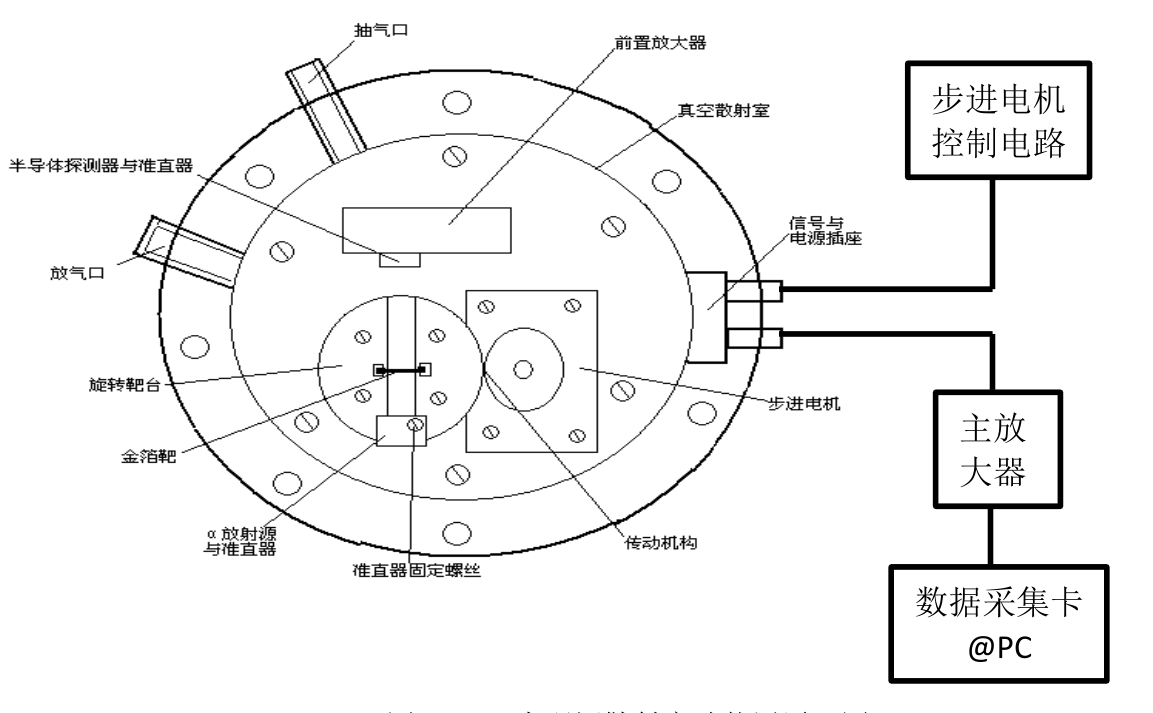
\includegraphics[width=0.8\textwidth]{./fig_apparatus.png}
        \caption{卢瑟福散射实验装置原理图}
    \end{minipage}
\end{figure}

散射真空室中主要包括有$\alpha$放射源、散射样品台、$\alpha$粒子探测器、步进电机及转动机构等。放
射源为$^{241}Am$源,$^{241}Am$源主要的$\alpha$粒子能量为$5.486MeV$。

在本实验装置中利用步进电机来控制散射角$\theta$可使实验过程变得极为方便。不用每测
量一个角度的数据便打开真空室转换角度,只需在真空室外控制步进电机转动相应的角度即可。

数据采集系统前端的$\alpha$粒子探测器为金硅面垒Si(Au)探测器,此外还有电荷灵敏前置放大器、
主放大器、探测器电源、NIM机箱与数据采集卡。其中前置放大器和主放大器用于将探测器输出的
信号放大到合适的幅度,再由数据采集卡对信号进行分析处理。

\section{实验内容}

\begin{enumerate}
    \item 观察真空室结构及靶台的旋转控制,并且进行一些物理量的标定。
    \item 测量$\alpha$粒子束的强度及在空气中的射程,计算$\alpha$粒子的能量E
    \item 验证$N \propto \frac{1}{\sin^4{\frac{\theta}{2}}}$
\end{enumerate}

\section{实验数据及处理分析}

\subsection{原始实验数据}

\subsubsection{一些测量初始值}

\begin{enumerate}
    \item 靶到探头的距离,$l_1$ = 3.75cm + 0.2cm = 3.95 cm
    \item 源到探头的距离,$l_2$ = 6.65cm + 0.2cm = 6.85 cm
    \item $T$ = $19 ^\circ C$ 
\end{enumerate}

以下所有数据的记录,都是在感兴趣区(ROI)范围为200-1000的地方取值。

\subsubsection{空气靶}

\begin{table}[H]
    \centering
    \begin{tabular}{|c|c|c|c|c|c|c|c|}
    \hline
        $\theta$ & $-5^{\circ}$ & $-4^{\circ}$ & $-3^{\circ}$ & $-2^{\circ}$ & $-1^{\circ}$ & $0^{\circ}$ & $1^{\circ}$ \\ \hline
        N & 76773 & 88479 & 91076 & 86569 & 77171 & 64019 & 46754 \\ \hline
    \end{tabular}
    \caption{空气靶时角度与入射粒子数的关系表}
\end{table}

以上数据的测量时间为60s。

得出此时物理$0^\circ$角为$-3^\circ$角,接下来于物理$0^\circ$角继续进行测量。

\begin{table}[H]
    \centering
    \begin{tabular}{|c|c|c|c|c|c|c|}
    \hline
        P(kPa) & 0 & 6 & 12 & 18 & 24 & 30 \\ \hline
        N & 181109 & 160884 & 145866 & 125394 & 97962 & 68592 \\ \hline
    \end{tabular}
    \caption{空气靶$\theta=0$时P与入射粒子数的关系表}
\end{table}

以上数据的测量时间为120s

\subsubsection{金靶}

\begin{table}[H]
    \centering
    \begin{tabular}{|c|c|c|c|c|c|c|c|c|}
    \hline
        $\theta$ & $-3 ^\circ$ & $-2 ^\circ$ & $-1 ^\circ$ & $0^\circ$ & $1 ^\circ$ & $2 ^\circ$ & $3 ^\circ$ & $4^\circ$ \\ \hline
        N & 11364 & 12742 & 13800 & 14672 & 14946 & 14998 & 14523 & 13832 \\ 
        N部分第二次测量 & ~ & ~ & ~ & ~ & 14972 & 15157 & ~ & ~ \\ \hline
    \end{tabular}
    \caption{金靶时角度与入射粒子数的关系表}
\end{table}

以上数据的测量时间为90s

可得此时物理$0^\circ$角为$2^\circ$角,接下来于物理$0^\circ$角进行测量

\begin{table}[H]
    \centering
    \begin{tabular}{|c|c|c|c|c|c|}
    \hline
        $\theta$ & $10^\circ$ & $13^\circ$ & $16^\circ$ & $19^\circ$ & $22^\circ$ \\ \hline
        t(s) & 150 & 200 & 400 & 600 & 800 \\ \hline
        N & 5722 & 3510 & 3102 & 2085 & 1255 \\ \hline
    \end{tabular}
    \caption{金靶时特定角度与特定时间时入射粒子数的关系表}
\end{table}

\subsection{数据的处理}

\subsubsection{空气靶}

由卢瑟福散射公式得:

\begin{equation}
    N = \frac{dn}{nN_{0}td\Omega} = (\frac{1}{4\pi \epsilon_{0}})^2 (\frac{2Ze^2}{4E})^2 nN_0t \frac{\Omega}{\sin^4{\frac{\theta}{2}}}
\end{equation}

于低真空环境中,可以将腔内的气体近似为理想气体,满足克拉伯龙方程:

\begin{equation}
    P = nkT
\end{equation}

联立上面2式可得:

\begin{equation}
    N = \frac{dn}{nN_{0}td\Omega} = (\frac{1}{4\pi \epsilon_{0}})^2 (\frac{2Ze^2}{4E})^2 \frac{N_0 t P}{k T} \frac{\Omega}{\sin^4{\frac{\theta}{2}}}
\end{equation}

当角度确定时,上式可以近似为:

\begin{equation}
    N = const \cdot \frac{P}{T}
\end{equation}

即当温度相同时,N,P呈线性关系,所以采用最小二乘法的线性拟合。

得到拟合公式为:

\begin{equation}
    N = 185098.048 -3675.348 P(kPa)
\end{equation}

\begin{figure}[H]
    \centering
    \begin{minipage}[b]{0.9\textwidth}
        \centering
        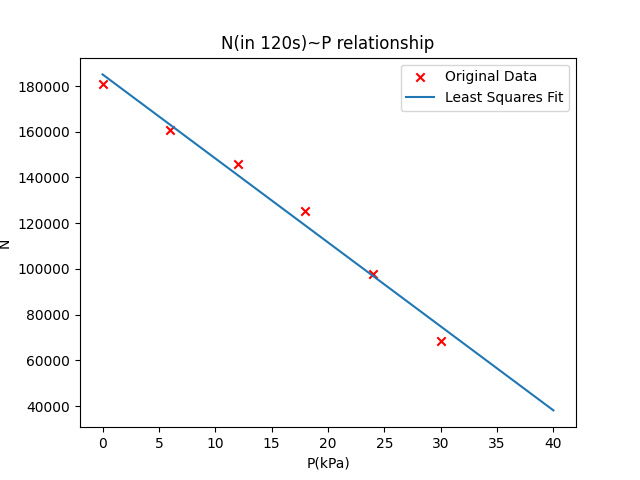
\includegraphics[width=0.8\textwidth]{./np.png}
        \caption{120s内接受到的粒子数N与空气压强P的关系图}
    \end{minipage}
\end{figure}

可知初始强度于$P=0$时,散射粒子时为0,此时取到120s内接收的总粒子数为185098,得$N_0 = \frac{185098}{120} = 1542.483$

当$N = \frac{1}{2}N_0$时,$P_{\frac{1}{2}} = 25.181 kPa$,此时计数率降为一半,此时的
射程为平均射程$R_{\frac{1}{2}} = l_2 + 2mm$

由此通过关系式:

\begin{equation}
    P_{\frac{1}{2}}R_{\frac{1}{2}} \frac{1}{T_{\frac{1}{2}}} = P_{1}R_{1} \frac{1}{T_1}
\end{equation}

其中$R_{\frac{1}{2}} = l_2 = 6.85cm$,$T_{\frac{1}{2}}=273.15 + 19 = 292.15K$,$T_1 = 273.15K$

得:

\begin{equation}
    R_{1} = \frac{P_{\frac{1}{2}}R_{\frac{1}{2}}}{P_1} \cdot \frac{T_1}{T_{\frac{1}{2}}}= \frac{25.181}{101.325}\cdot \frac{273.15}{292.15} \cdot 6.85cm = 1.592cm
\end{equation}

所以,动能为$5.486MeV$的$\alpha$粒子于$0^\circ C$,一个标准大气压下的射程R为1.592cm。

由于$E \approx 5.486 MeV$,所以,由计算公式近似可得:

\begin{equation}
    R = (0.285+0.005E)E^{\frac{3}{2}} \cong 0.285E^{\frac{3}{2}}
\end{equation}

所以有:

\begin{equation}
    E = (\frac{R}{0.285})^{\frac{2}{3}} = 3.148 MeV
\end{equation}

\subsubsection{金靶}

\begin{table}[H]
    \centering
    \begin{tabular}{|c|c|c|c|c|c|}
    \hline
        $\theta$ & $10^\circ$ & $13^\circ$ & $16^\circ$ & $19^\circ$ & $22^\circ$ \\ \hline
        $\sin^4{\frac{\theta}{2}}$ & $5.770 \times 10^{-5}$ & $1.642 \times 10^{-4}$ & $3.752 \times 10^{-4}$ & $7.421 \times 10^{-4}$ & $1.326 \times 10^{-3}$ \\ \hline
        $\frac{1}{\sin^4{\frac{\theta}{2}}}$ & 17330.7 & 6089.27 & 2665.5 & 1347.61 & 754.405 \\ \hline
        N/t & 38.147 & 17.55 & 7.755 & 3.475 & 1.569 \\ \hline
        K & $2.201 \times 10^{-3}$ & $2.882 \times 10^{-3}$ & $2.909 \times 10^{-3}$ & $2.579 \times 10^{-3}$ & $2.080 \times 10^{-3}$ \\ \hline
    \end{tabular}
    \caption{金靶时特定角度与单位时间入射粒子数,K值的关系表}
\end{table}

先验证卢瑟福散射公式$N/t \propto \frac{1}{\sin^4{\frac{\theta}{2}}}$,做$N/t \sim \frac{1}{\sin^4{\frac{\theta}{2}}}$图。

\begin{figure}[H]
    \centering
    \begin{minipage}[b]{0.9\textwidth}
        \centering
        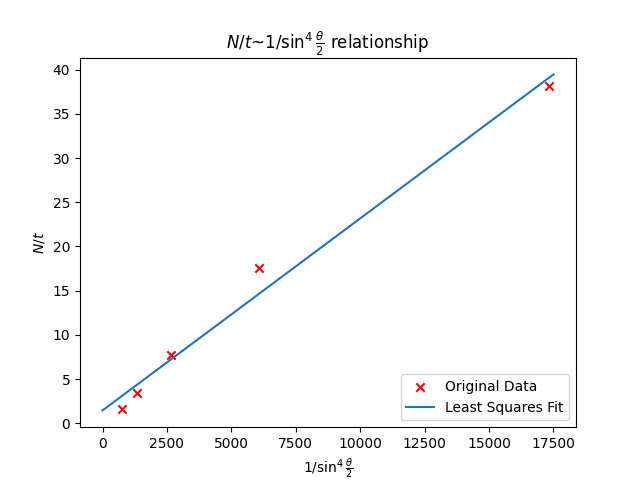
\includegraphics[width=0.8\textwidth]{./r.png}
        \caption{单位时间内接受到的粒子数$N/t$与$\frac{1}{\sin^4{\frac{\theta}{2}}}$的关系图}
    \end{minipage}
\end{figure}

拟合其关系式为:

\begin{equation}
    N/t = 1.454 + 2.172 \times 10^{-3} \frac{1}{\sin^4{\frac{\theta}{2}}}
\end{equation}

由上式可以得出K的拟合值为$K = 2.172 \times 10^{-3}$

下面由公式给出K的理论值:

\begin{equation}
    K = 4.8065 \times 10^{-34} \frac{N_0}{E^2 l_{1}^2} = 4.8065 \times 10^{-34} \frac{1542.48}{(3.148 MeV \times 0.0395m)^2} = 1.868 \times 10^{-3}
\end{equation}

K于前4个节点的真实值与理论值相差较大,与最后一个节点较为接近。

下面给出$K \sim \theta$曲线,由于K理论上为一个常数,故利用直线对$K \sim \theta$进行拟合:

\begin{figure}[H]
    \centering
    \begin{minipage}[b]{0.9\textwidth}
        \centering
        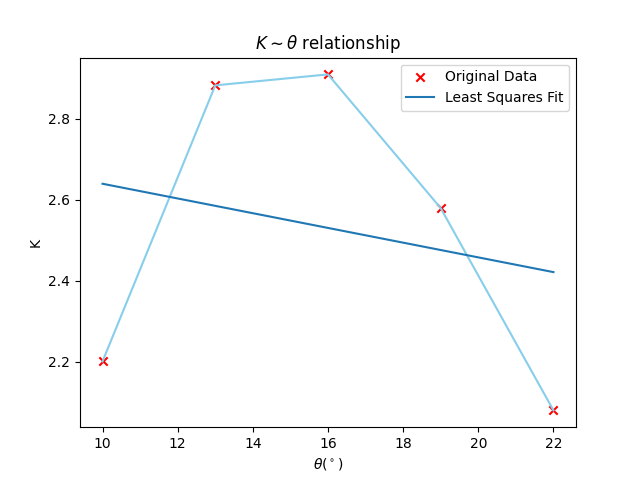
\includegraphics[width=0.8\textwidth]{./k.png}
        \caption{$K$与$\theta$的关系图}
    \end{minipage}
\end{figure}

得出的拟合曲线为:

\begin{equation}
    K = 2.821 \times 10^{-3} - 0.018 \theta
\end{equation}

由于采样点有限,所以只能用最小二乘法对数据进行拟合,发现得到的结果与之前的结果存在差异。

\section{实验总结和误差分析}

\subsection{实验总结}

\begin{enumerate}
    \item 测量出的单位时间内放射源发射的$\alpha$粒子的数量为$N_0 = 1542.5 s^{-1}$
    \item 计算出$\alpha$粒子在$0^\circ C,1 atm$的条件下的射程为$R = 1.592 cm$,计算得此放射源出射$\alpha$粒子的能量为$E = 3.148 MeV$
    \item 此实验中分析的理论K值为$1.868 \times 10^{-3}$,获得的K值的拟合值为$2.172 \times 10^{-3}$,把每一对测量值单独计算得的K值与拟合值与理论值对比,发现相差较大。
\end{enumerate}

\subsection{误差分析}

首先需要指出的一点是:实验中的$\alpha$粒子能量测量值与实验讲义上给出的内容有所出入,由于实验的测量点有限,在这种情况下不能进行准确的判断,
在以下的讨论中,更倾向于认为实验测得的值是较为准确的。

\begin{enumerate}
    \item E与理论值的差异,在假设实验测得值准确的前提下,认为可能的原因是放射源已经有部分衰变,导致强度下降;若假设理论正确,则实验中出现的问题可能是实验中的低真空装置存在误差,
    由于无法达到严格的低真空,所以测得的平均误差偏小,导致测得的$\alpha$粒子偏小。
    \item 关于K值的计算,理论计算值为$1.868 \times 10^{-3}$,实验拟合值为$2.172 \times 10^{-3}$,这两者较接近,但与各个测量点的直接计算值相差较大,于$13^\circ,16^\circ,19^\circ$尤为明显。
    可能的原因是有两个,一个原因是总体的采样值个数较少,于几个比较大的角度,采样得的粒子数仅有几千个,由中心极限定理的条件估计,误差较大;第二个原因可能是由于测量的角度值的数目有限,需要用
    最小二乘法进行拟合来减小误差,直接比较没有太大意义。
\end{enumerate}

\section{思考题}

\subsection{根据卢瑟福公式$N\sin^4{(\frac{\theta}{2})}$应为常数,本实验的结果有偏差吗?试分析原因。}

有偏差,$N\sin^4{(\frac{\theta}{2})} = K$。在上面的分析得,K值在角度$13^\circ,16^\circ,19^\circ$时,偏差较大;而在角度$10^\circ,22^\circ$时,偏差较小。分析的原因于本页6.2误差分析中的第二点。下面重新给出:

关于K值的计算,理论计算值为$1.868 \times 10^{-3}$,实验拟合值为$2.172 \times 10^{-3}$,这两者较接近,但与各个测量点的直接计算值相差较大,于$13^\circ,16^\circ,19^\circ$尤为明显。
    可能的原因是有两个,一个原因是总体的采样值个数较少,于几个比较大的角度,采样得的粒子数仅有几千个,由中心极限定理的条件估计,误差较大;第二个原因可能是由于测量的角度值的数目有限,需要用
    最小二乘法进行拟合来减小误差,直接比较没有太大意义。

\subsection{若人体肌肉组织的密度为$1.10g/cm^3$,根据实验内容4的结果估算本实验中的$\alpha$粒子在
人体肌肉组织中的射程,单位取$cm$。}

由之前的讨论可得:

\begin{equation}
    \rho_{air} R_{air} = \rho_{human} R_{human} 
\end{equation}

代入$0^{\circ}C, 1 atm$时$\rho_{air} = 1.293 Kg/m^3$,$R_{air} = 1.592cm$,$\rho_{human} = 1100 Kg/m^3$,得:

\begin{equation}
    R_{human} = \frac{\rho_{air}R_{air}}{\rho_{human}} = 1.871 \mu m
\end{equation}

可得本实验中的$\alpha$粒子在人体肌肉组织中的平均射程为$1.871 \mu m$。需要注意的是,此处的平均射程具有统计意义。

\end{document}